\documentclass[final,hyperref={pdfpagelabels=false}]{beamer}

\usepackage[orientation=portrait,size=a0,scale=1.13,22pt]{beamerposter} % Use the beamerposter package for laying out the poster with a portrait orientation and an a0 paper size
\usepackage[backend=biber, style=numeric, citestyle=numeric]{biblatex}
%\usepackage{fontenc}
\usepackage{units}
\usepackage{siunitx}
\usepackage{graphicx}
\usepackage{graphicx, caption, subcaption}
\usepackage{geometry,array,graphicx,float,caption}
\usepackage{subcaption}
\usepackage[version=3]{mhchem} % Formula subscripts using \ce{}
\usepackage{physics}
\usepackage[T1]{fontenc}
\usepackage[sfdefault]{FiraSans}
\usepackage{newtxsf}

\newcommand{\cref}{c^{\ominus}}
\newcommand{\Hplus}{\text{H}^{+}}
\newcommand{\Aminus}{\text{A}^{-}}
\usetheme{I6pd2} % Use the I6pd2 theme supplied with this template
\usepackage[english]{babel} % English language/hyphenation
\usepackage{amsmath,amsthm,amssymb,latexsym} % For including math equations, theorems, symbols, etc
\usepackage{subcaption}
\usepackage{booktabs} % Top and bottom rules for tables
\graphicspath{{figures/}} % Location of the graphics files
\usepackage[backend=biber, style=numeric, citestyle=numeric]{biblatex}
\usecaptiontemplate{\structure{\insertcaptionname~\insertcaptionnumber: }\insertcaption} % A fix for figure numbering

%----------------------------------------------------------------------------------------
%	TITLE SECTION 
%----------------------------------------------------------------------------------------
\title{\textbf{\HUGE {\textcolor{dblue}{Quantum Criticality} in Long Range Transverse Field Ising Model}}} % Poster title 
\vspace{-5.5cm}
\author{\LARGE{Devashish Tiwari$^{1}$} \& Auditya Sharma$^1$} %
\institute{\textit{\large $^1$Department of Physics, Indian Institute of Science Education and Research, Bhopal, India}}
\usepackage{tikz}
\usetikzlibrary{tikzmark}
%\usetikzlibrary{shapes,snakes}
\setbeamertemplate{background canvas}{%
\begin{tikzpicture}[remember picture,overlay]
\shade[top color=white,bottom color=hblue, shading angle=0]
  ([shift={(0.0cm,0.0cm)}]current page.north west)
     rectangle
  ([shift={(0.0cm,0.0cm)}]current page.south east);
\end{tikzpicture}%     
}
\begin{document}
\addtobeamertemplate{block end}{}{\vspace*{2ex}} % White space under blocks
\begin{frame}[t] % The whole poster is enclosed in one beamer frame

\begin{columns}[t] 

\begin{column}{.48\textwidth} % The first column

\begin{block}{Abstract}
\item The critical behavior of many quantum systems, like the long-range transverse field Ising model, is not well understood in terms of quantum correlation measures like entanglement entropy because of the lack of efficient computational methods. Projector Quantum Monte Carlo (PQMC), well-established for short-range models, is extended here to the long-range case to comment on the behavior of critical exponents and entanglement entropy at criticality in the thermodynamic limit $L \xrightarrow[]{} \infty$. \\
\end{block}

\begin{block}{Quantum Monte Carlo Methods}
\textbf{Classical Monte Carlo:}
\begin{itemize}
    \item The classical partition function is:
    \begin{align}
        Z = \sum_{i} e^{-\beta E_i}.
    \end{align}
    \item One samples each term of this expansion in the simulation, and extracts observables: 
    \begin{align}
        \langle O \rangle  = \sum_{i}\frac{O_i e^{-\beta E_i}}{Z}.
    \end{align}
\end{itemize}
\text{ }\\
\textbf{Quantum Monte Carlo (Stochastic Series Expansion)} \cite{1}:
\begin{itemize}
\item Quantum partition function is the trace over the thermal density matrix.
\begin{align}
   Z &= \operatorname{Tr}(\hat{\rho}) = \operatorname{Tr}(\mathrm{e}^{-\beta \hat{H}}),
\end{align}
\begin{align}
    Z &= \sum_{\alpha_{0}} \langle \alpha_{0} \mid \mathrm{e}^{-\beta \hat{H}} \mid \alpha_{0} \rangle = \sum_{\alpha_{0}} \sum_{n = 0}^\infty \frac{(-\beta)^{n}}{n!} 
    \langle \alpha_{0} \mid \hat{H}^n \mid \alpha_{0} \rangle,
\end{align}
\begin{align}
    Z = \sum_{n = 0}^\infty \sum_{{\{\alpha\}}}\frac{(-\beta)^{n}}{n!} &\langle \alpha_{0} \mid \hat{H} \mid \alpha_{1} \rangle 
    \langle \alpha_{1} \mid \hat{H} \mid \alpha_{2} \rangle \notag \cdots \langle \alpha_{n-1} \mid \hat{H} \mid \alpha_{0} \rangle \label{eq:monte_carlo_sum}.
\end{align}
%One can add a more complete set of identities:
%\begin{align}
 %   Z = \sum_{n = 0}^{M} \sum_{\{\alpha\}} \frac{(-\beta)^n (M - n)!}{M!} 
 %   &\langle \alpha_{0} \mid {\hat{H}} \mid \alpha_{1} \rangle 
 %   \langle \alpha_{1} \mid {\hat{H}} \mid \alpha_{2} \rangle \notag \cdots \langle %\alpha_{M-1} \mid {\hat{H}} \mid \alpha_{0} \rangle \label{eq:modi_monte_carlo_sum}.
%\end{align}
\item If the Hamiltonian is a local operator, then
\begin{equation}
     Z = \sum_{n = 0}^{M} \sum_{\{\alpha\}} \frac{(-\beta)^n (M - n)!}{M!} \prod_{m = 1}^M \langle \alpha_{m-1} \mid \hat{H}_{t_m, a_m} \mid \alpha_{m} \rangle . \label{eq:final_partition_function_sample}
\end{equation}
\end{itemize}
\text{ }\\
\begin{figure}
    \centering
    \includegraphics[width=0.6\linewidth]{2023-tiwari-espresso-summer-school-poster-session-pimd-main//figures/projector_image.pdf}
    \caption{$(D + 1)$-dimensional representation of a configurational cell in SSE}
\end{figure}
\textbf{Projector Quantum Monte Carlo}:
\begin{itemize}
\item To obtain $T = 0$ expectation values, one can increase $\beta$ but this is computationally costly. Instead, the projector method achieves faster convergence.
\begin{equation}
    \left( -\hat{H} \right)^m \mid \alpha_d \rangle = c_0 |E_0|^m \left( |0\rangle + \frac{c_1}{c_0} \left( \frac{E_1}{E_0} \right)^m |1\rangle + \cdots \right).
\end{equation}
\item Then, the partition function at $T = 0$ is:
\begin{align}
    Z &= \sum_{\{\alpha\}} \langle \alpha_k \mid (-\hat{H})^p(-\hat{H})^{r} \mid \alpha_d \rangle = \sum_{\{\alpha\}} \sum_{S_{r + p}} \prod_{j = 1}^{r + p}\langle \alpha_k \mid (-\hat{H}_{t_j, a_j}) \mid \alpha_d \rangle.    
\end{align}
\end{itemize}
\end{block}

\begin{block}{Transverse Field Ising Model}
\textbf{Paradigmatic Model for Quantum Phase Transitions}
\begin{itemize}
    \item This model exhibits an order-disorder transition at $T = 0$ in all dimensions:
    \begin{equation}
        \hat{H} = -J \sum_{i} \sigma_{i}^{z} \sigma_{i + 1}^{z} - h^T \sum_{i} \sigma_{i}^{x},  
        \label{eq:Hamiltonian_TFIM}
    \end{equation}
    where $J$ is the interaction strength and $h^T$ is the transverse field.  
\end{itemize}

\begin{columns}[T,onlytextwidth]
\column{0.5\textwidth} 
\begin{figure}[H]
\centering
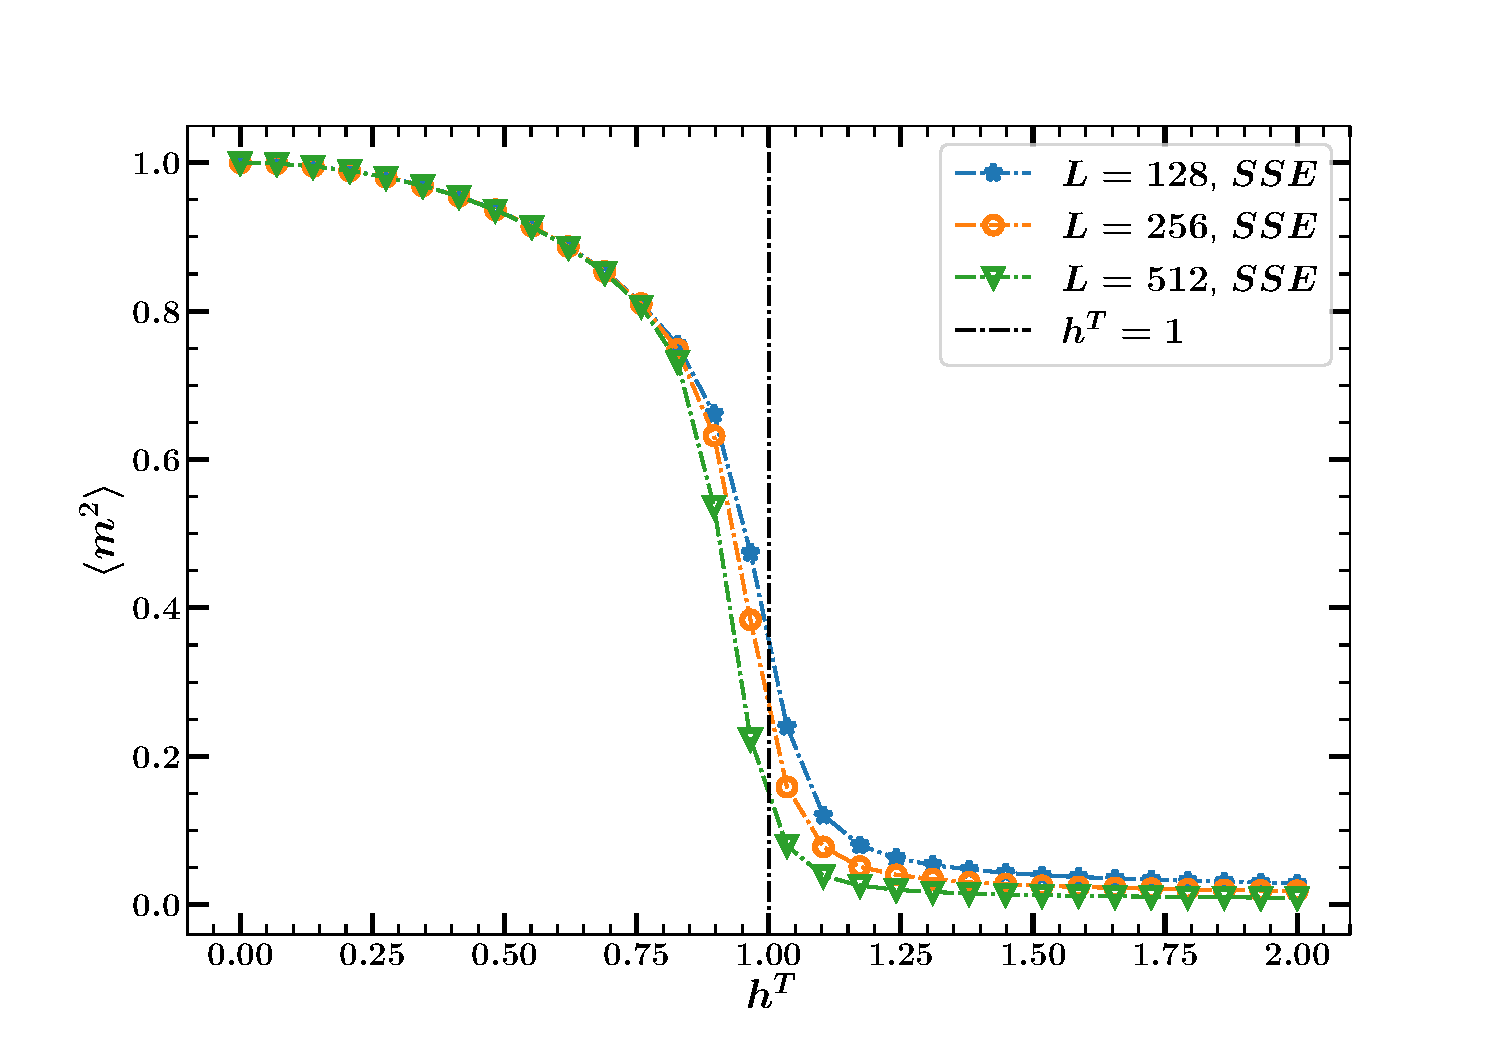
\includegraphics[width=0.9\textwidth]{2023-tiwari-espresso-summer-school-poster-session-pimd-main/figures/magnetization_ground_state.pdf}
\caption{$\langle m^2 \rangle$ for 1D TFIM at $T = 0$.}
\end{figure}
\column{0.5\textwidth} 
\begin{figure}[H]
\centering
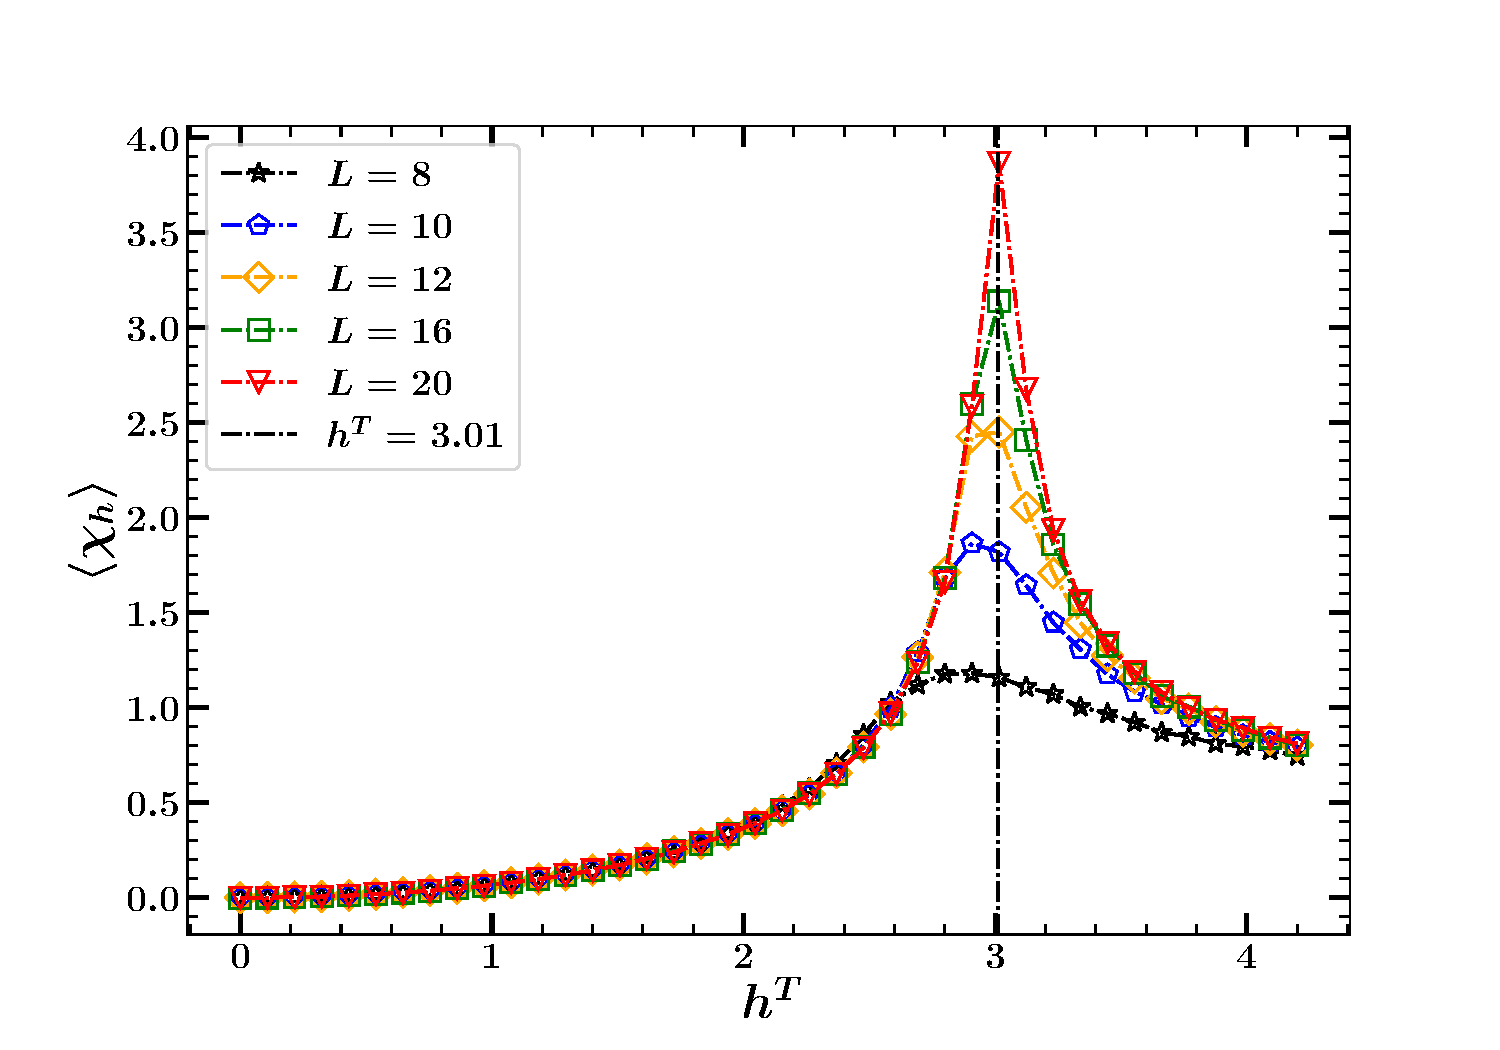
\includegraphics[width=0.9\textwidth]{2023-tiwari-espresso-summer-school-poster-session-pimd-main/figures/susceptibility_2d_tfim_zero_temp.pdf}
\caption{Susceptibility for 2D TFIM at $T = 0$.}
\end{figure}
\end{columns}
\end{block}
\end{column} % End of the first column
\begin{column}{.48\textwidth}

\begin{block}{Long Range Interactions}
\begin{itemize}
\item Model system -- 1D Long Range Transverse Field Ising Model (LRTFIM):
\begin{equation}
\hat{H} = -\sum_{i, j} \frac{J}{r^{d + \sigma}} \sigma_{i}^{z} \sigma_{j}^{z} - h^T \sum_{i} \sigma_{i}^{x},  \label{eq:Hamilotnian_TFIM} 
\end{equation}
where $d$ is the system's dimension and $\sigma$ is a parameter tuning the interaction range.
\end{itemize}
\begin{columns}[T,onlytextwidth]
\column{0.5\textwidth} 
\begin{figure}[H]
\centering
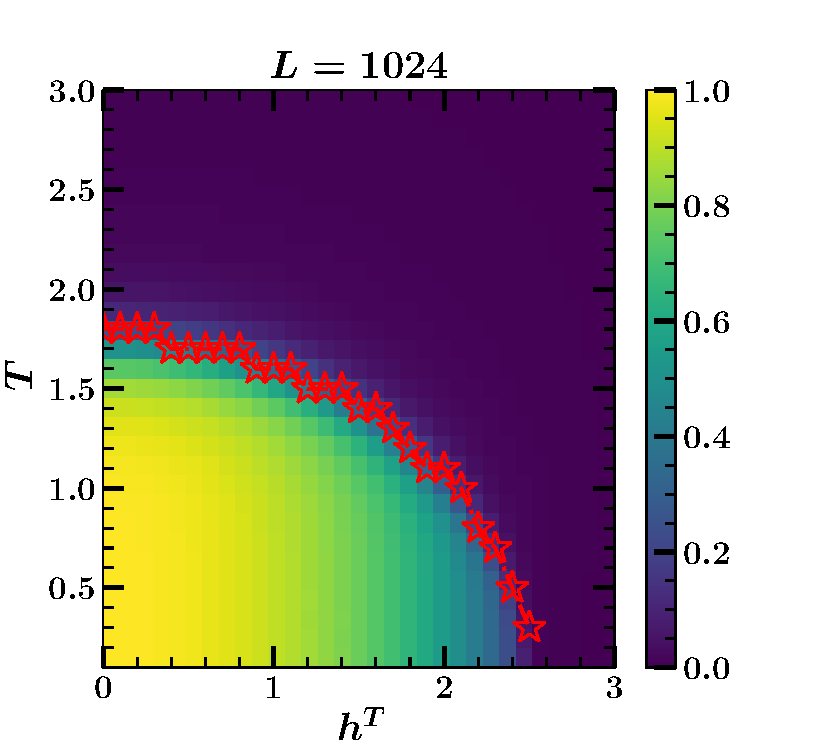
\includegraphics[width=0.9\textwidth]{2023-tiwari-espresso-summer-school-poster-session-pimd-main/figures/dyson_moel_sigma_1_transverse_field_phase_transitions.pdf}
\caption{$\langle m^2 \rangle$ from finite-$T$ SSE (KT transition)}
\end{figure}

\column{0.5\textwidth} 
\begin{figure}[H]
\centering
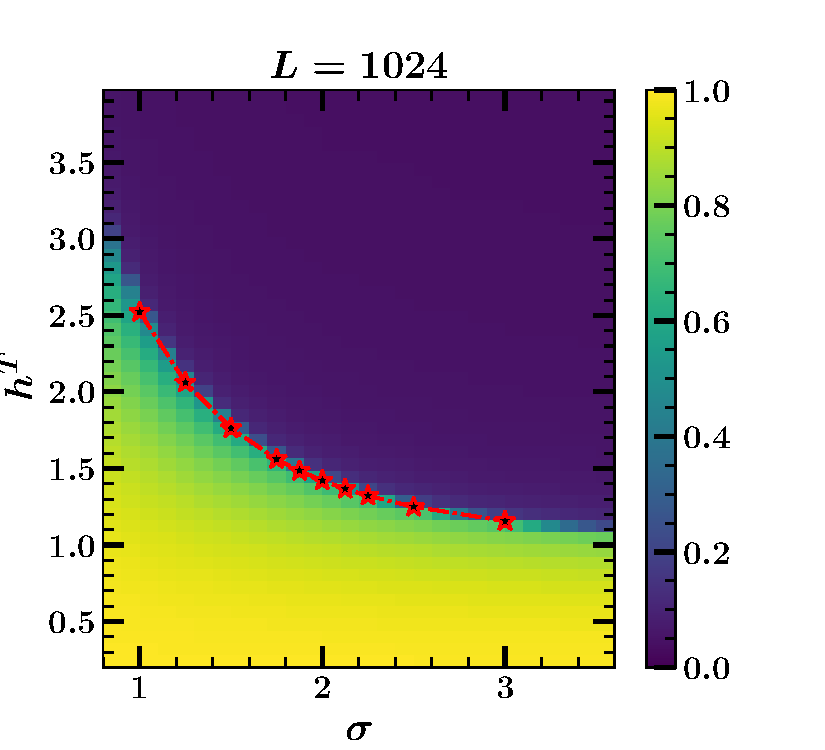
\includegraphics[width=0.9\textwidth]{2023-tiwari-espresso-summer-school-poster-session-pimd-main/figures/zero_temp_lrtfim_study_h_sigma.pdf}
\caption{$\langle m^2 \rangle$ from PSSE}
\end{figure}
\end{columns}
\end{block}

\begin{block}{Entanglement Entropy}

\begin{itemize}
\item Entanglement is a useful quantity to detect quantum phase transitions.
\item In SSE, the second-order Rényi entropy is computed via the replica trick:  
\begin{equation}  
S_A^{(2)} = -\ln \text{Tr}(\rho_A^2) = -\ln \langle SWAP_A \rangle,  
\end{equation}  
where \(\langle SWAP_A \rangle\) is the expectation value of the SWAP operator for subsystem \( A \) between two replicas.
\end{itemize}
\begin{columns}[T,onlytextwidth]
\column{0.5\textwidth} 
\begin{figure}[H]
\centering
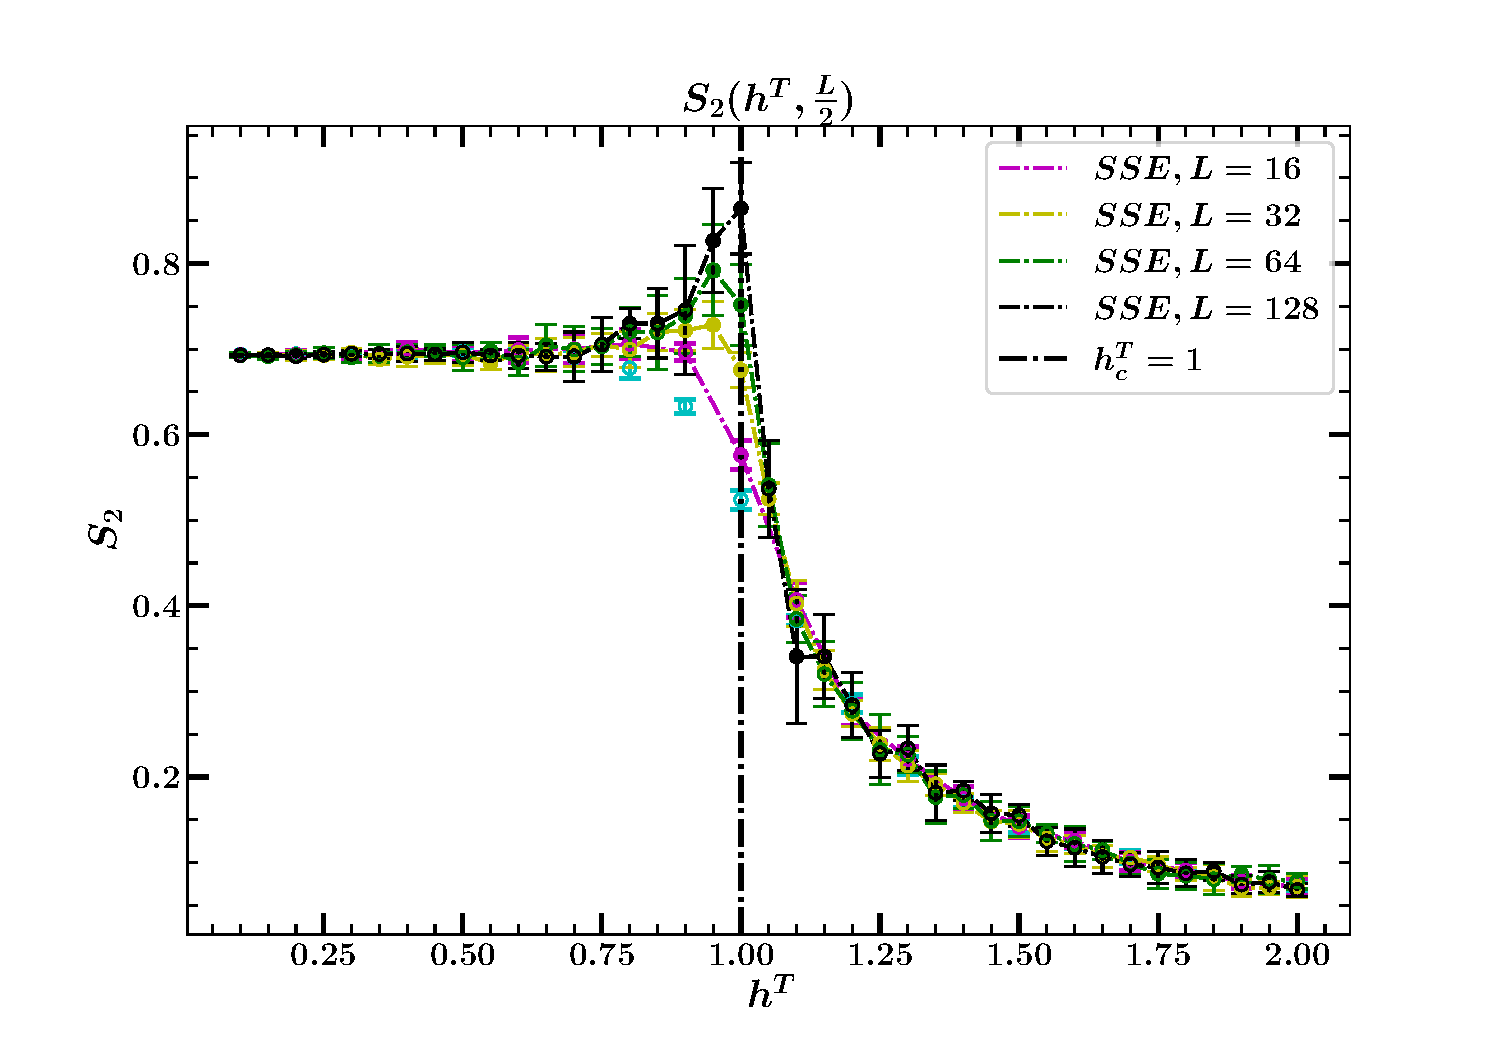
\includegraphics[width=1.0\textwidth]{2023-tiwari-espresso-summer-school-poster-session-pimd-main/figures/Entropy_SSE.pdf}
\caption{SRTFIM}
\end{figure}

\column{0.5\textwidth} 
\begin{figure}[H]
\centering
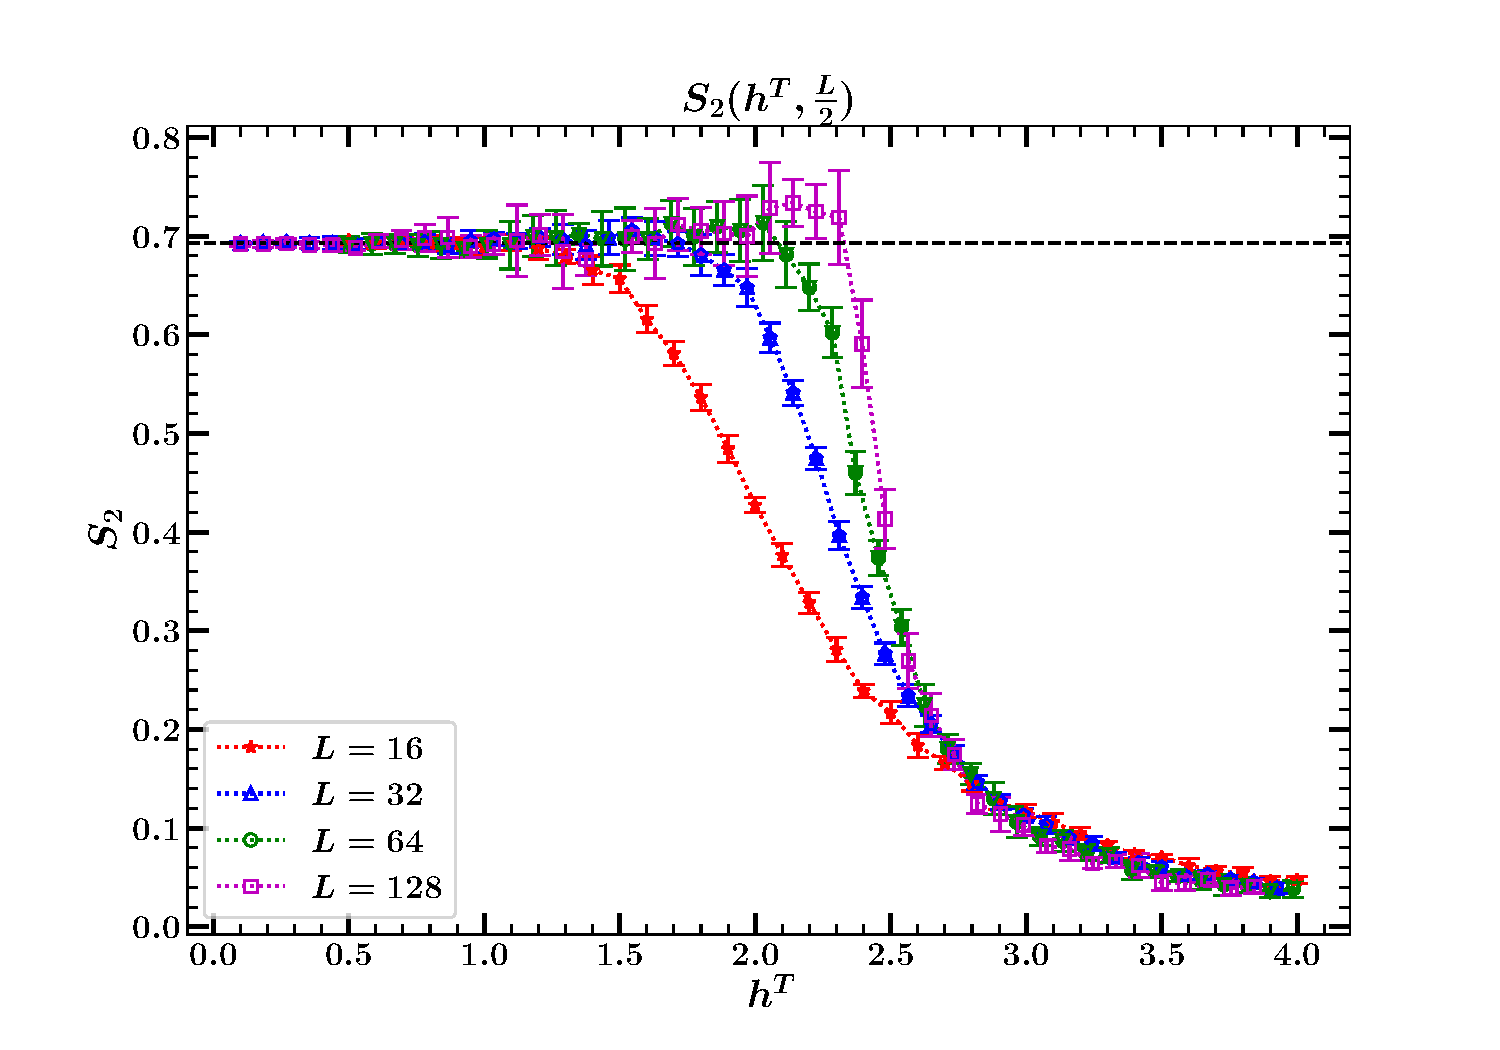
\includegraphics[width=1.0\textwidth]{2023-tiwari-espresso-summer-school-poster-session-pimd-main/figures/entropy_Lrtfim_ratio_trick_sigma_1.0.pdf}
\caption{LRTFIM with $\sigma = 1.0$}
\end{figure}
\end{columns}
\begin{itemize}
    \item \textbf{Area Law:} In SRTFIM, entanglement entropy scales as $L^{d - 1}$ outside criticality. These signatures still persists in long range interactions. 
\end{itemize}
\begin{figure}[H]
\centering
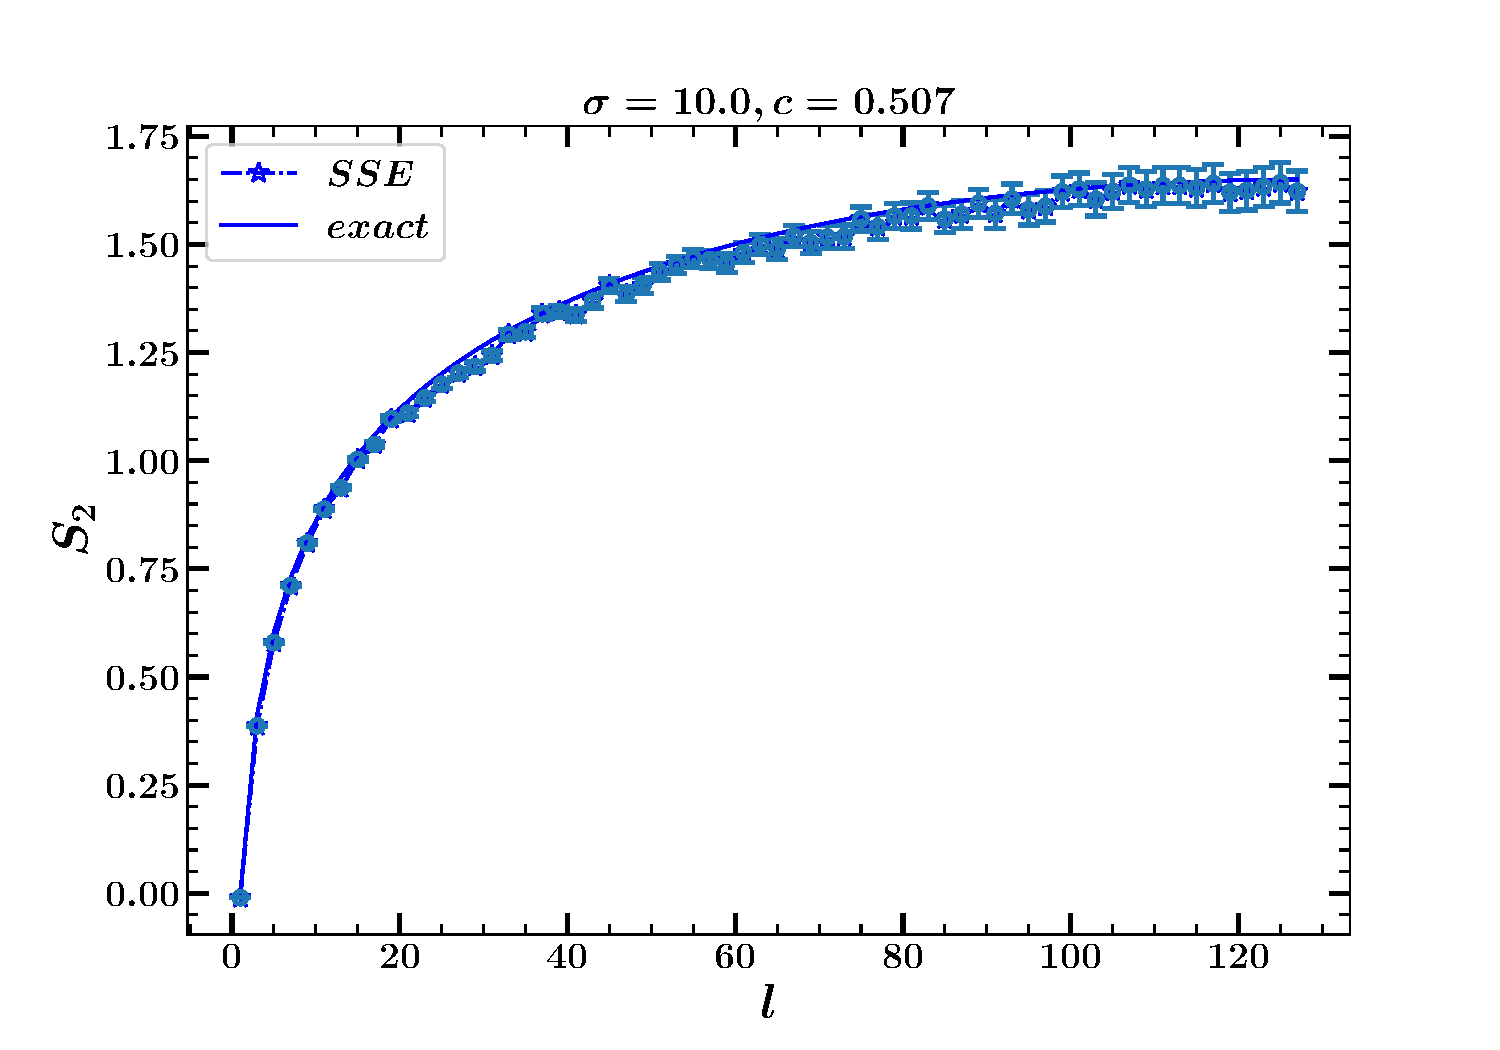
\includegraphics[width=0.5\textwidth]{2023-tiwari-espresso-summer-school-poster-session-pimd-main/figures/entanglement_entropy_logarithmic_violations_critical_magnetic_fidlf_h_equal_1.pdf}
\caption{Area law violations is logarithmic in short range regime\cite{3}}
\end{figure}
\end{block}


\begin{block}{Conclusion and Outlook}
\begin{itemize}
    \item Projector QMC allows us to obtain continuum results for the quantum model at $T = 0$.  
    \item The criticality in LRTFIM exhibits very distinct scaling behavior (in comparison to
SRTFIM), significantly affecting the behaviour of entanglement entropy area law. 
    \item Next step: to include the whole regime of long-range interactions, in order to accurately predict the robustness of the area law at the critical point.  
\end{itemize}
\end{block}

\vspace{-0.05cm}
\begin{block}{References}
\begin{thebibliography}{9}
\bibitem{1}
\textsc{Anders W. Sandvik}, 
\emph{Ground State Projection of Quantum Spin Systems in the Valence-Bond Basis}, 
Phys. Rev. Lett. \textbf{95}, 207203 (2010).

\bibitem{2}
\textsc{Matthew B. Hastings et al.}, 
\emph{Measuring Renyi Entanglement Entropy in Quantum Monte Carlo Simulations}, 
Phys. Rev. Lett. \textbf{104}, 157201 (2014).

\bibitem{3}
\textsc{Tomotaka Kuwahara et al.}, 
\emph{Area Law of Noncritical Ground States in 1D Long-Range Interacting Systems}, 
Nat. Commun. \textbf{11}, 4478 (2020).
\end{thebibliography}
\end{block}

\end{column}

\end{columns}

%------------------------------------------------------------------------------------
\end{frame} % End of the enclosing frame
\end{document}

